
% ════════════════════════════════════════════
% 模型准备（5.2.2.模型准备.tex，三级子块）
% ════════════════════════════════════════════
\subsubsection{模型准备}

\textbf{1.数据预处理}

附件二提供了 2025 年全年 365 天、每天 144 个 10 分钟时间点的小区负载与光伏实际功率数据，数据量约为 $365\times 144$ 的两张二维矩阵。为便于逐日建模，需要对数据进行时间对齐、数值化与按天切分。设第 $d$ 天第 $k$ 个间隔的负载与光伏功率分别为 $L_{d,k}$ 与 $S_{d,k}$，则全年数据可组织为：
\begin{equation}
    \boldsymbol{L}=[L_{d,k}]_{365\times 144},\quad \boldsymbol{S}=[S_{d,k}]_{365\times 144}
\end{equation}
其中，$d=0,1,\dots,364$ 表示天数序号，$k$ 表示日内间隔序号。对两张矩阵逐元素执行数值化检查，全年缺失值为零，负载分布于 $1995.7\sim 7978.9$ kW，光伏分布于 $0\sim 10216.2$ kW。需要说明的是，预处理阶段仅作时间对齐、按天切分与预测模型标定所必需的组织，不对真实功率序列作重采样、平滑与异常值替换，以免在数据中人为引入原始记录不具备的信息、掩盖真实的供需波动；预处理前后对比如图\ref{fig:preprocess2}所示。

\begin{figure}[H]
    \centering
    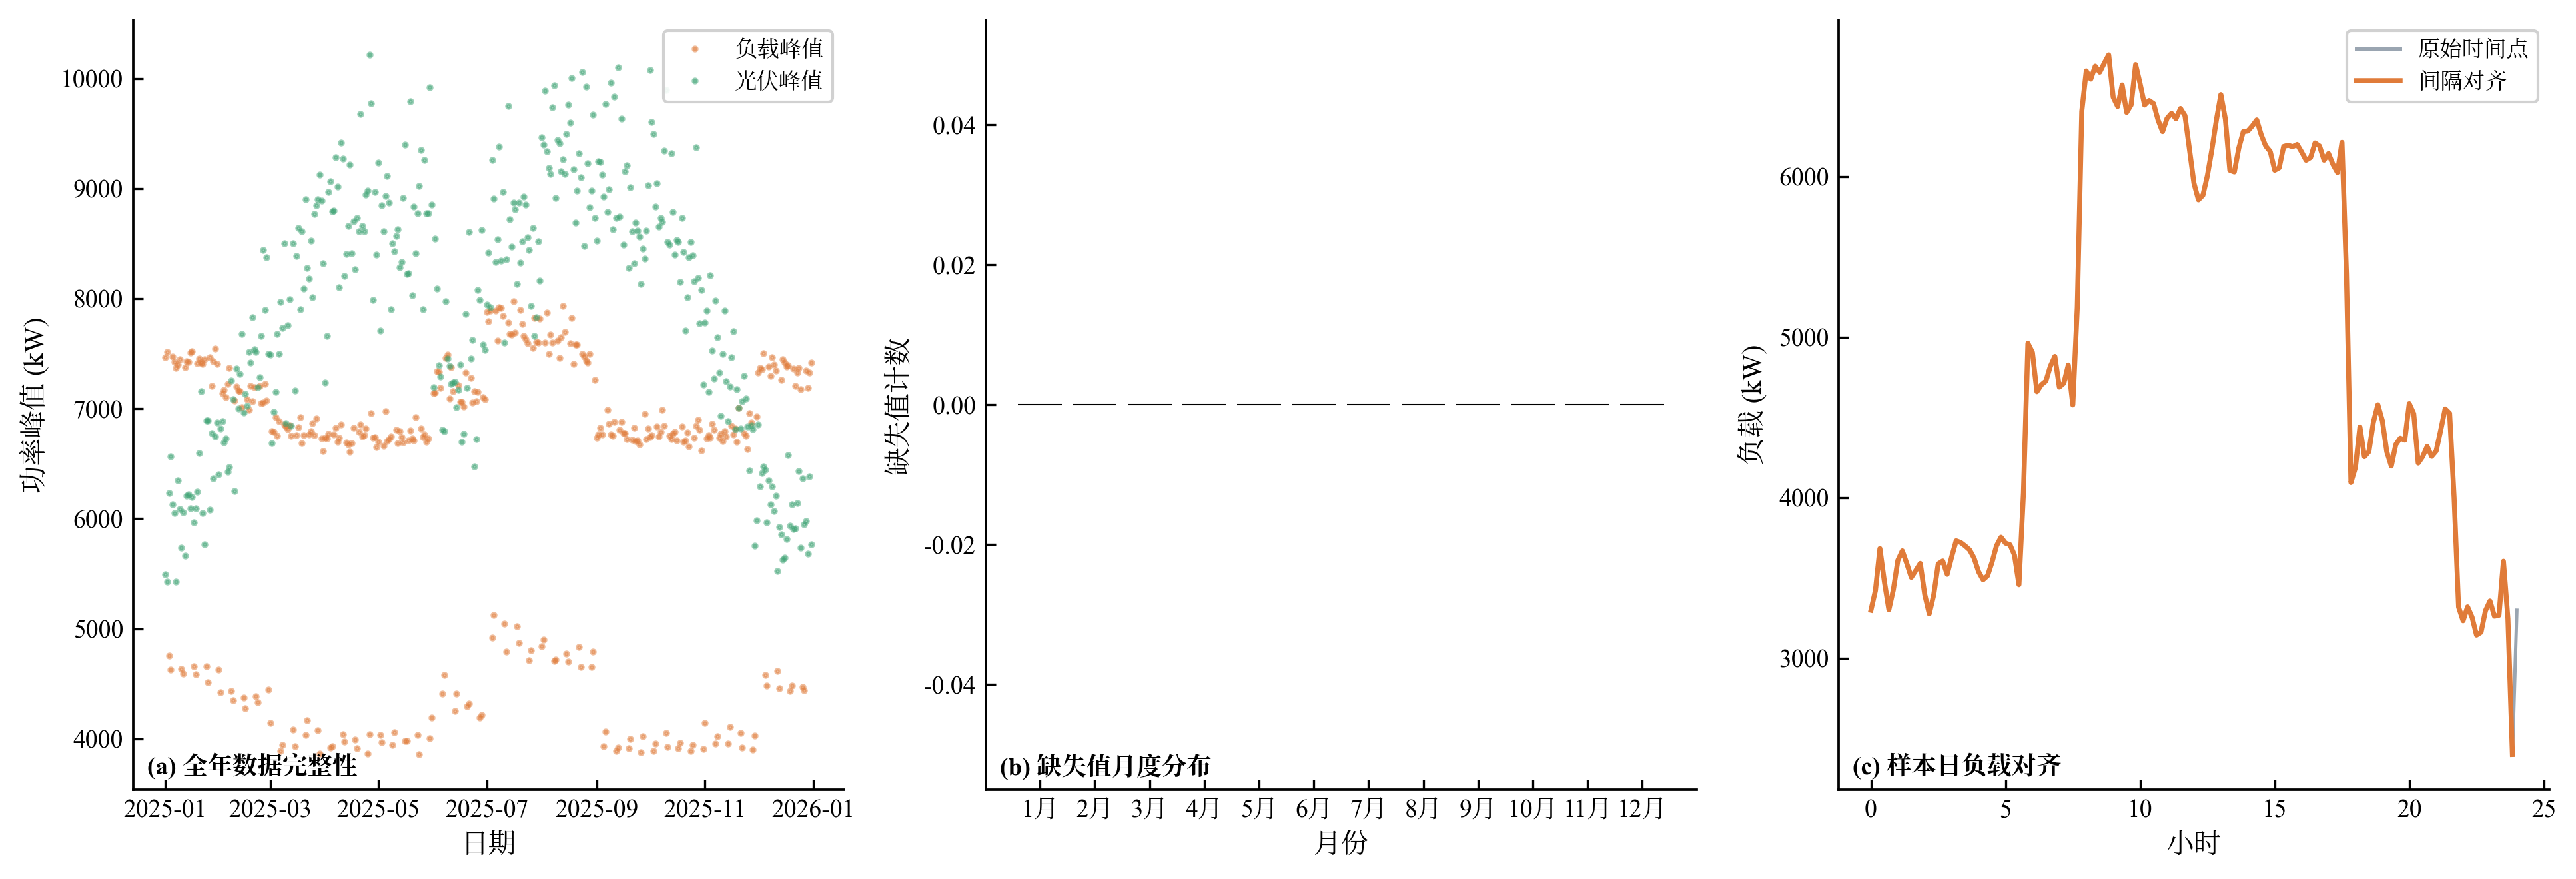
\includegraphics[width=0.72\textwidth]{求解/问题二/图片/图2-1_预处理前后对比.png}
    \caption{问题二全年数据预处理与完整性检查}
    \label{fig:preprocess2}
\end{figure}

由图\ref{fig:preprocess2}可知，全年负载与光伏峰值逐日变化，负载呈现明显的季节波动而光伏呈现冬低夏高的规律，且全年无缺失数据，样本日负载曲线在时间对齐后与原始时间点序列完全一致，数据质量良好。

需要说明的是，附件 2 的 365 天数据中，2025 年 1 月（1 月 1 日—1 月 31 日）承担\textbf{预热与训练双重作用}：一方面，模型以 1 月 1 日 0:00 储电量 6000 kWh 为初值逐日滚动，使储电量摆脱初始条件影响、进入稳定日循环（2 月 1 日 0:00 储电量已收敛至 1200 kWh 下限）；另一方面，1 月的实际功率与逐日预测残差被用于标定预测模型并估计其误差分布，是 2 月及以后各日制定计划的信息来源。由于 1 月不存在可用的历史信息，其自身按“无预测可用”处理（当天计划购电量取零、储能以初值支撑）。按照附件 5 的要求，结果文件与后文所有费用汇总均只统计 2025 年 2 月 1 日至 12 月 31 日共 334 天。

\textbf{2.算法选择}

在完成数据预处理后，本问需在预测不确定性的条件下完成 334 个逐日决策问题，其求解策略涉及两个层面的选择：一是同一日内计划量应当如何确定，二是全年 334 天之间应当如何组织。就第一点而言，当天的负载与光伏在 0:00 未知，若按预测值作确定性优化，则等于把预测误差全部当作不发生，会在 5 倍紧急电价下系统性低估缺电风险；若将预测误差离散为若干情景、令计划量对所有情景同时可行，并在目标中计入期望紧急购电费，则可得到对不确定性稳健的计划量，这正是\textbf{两阶段随机线性规划}的思想。就第二点而言，可从建模复杂度与最优性两个维度比较独立逐日求解与全年统一求解两种策略，如表\ref{tab:algo2}所示。

\begin{longtable}{>{\centering\arraybackslash}p{0.26\textwidth}>{\centering\arraybackslash}p{0.18\textwidth}>{\centering\arraybackslash}p{0.20\textwidth}>{\centering\arraybackslash}p{0.24\textwidth}}
  \caption{问题二求解策略对比}
  \label{tab:algo2} \\
  \toprule
  策略 & 建模复杂度 & 计算规模 & 最优性 \\
  \midrule
  \endfirsthead
  \caption{问题二求解策略对比（续）} \\
  \toprule
  策略 & 建模复杂度 & 计算规模 & 最优性 \\
  \midrule
  \endhead
  \bottomrule
  \endfoot
  全年统一求解 & 高 & 大规模 & 严格全局最优，但规划时须假定全年功率已知 \\
  逐日滚动确定性求解 & 低 & 小规模 & 本问条件下与全年统一最优等价，但忽略预测误差 \\
  逐日滚动随机规划（本文采用） & 中 & 小规模 $\times$ 9 情景 & 计划量不含事后信息，紧急购电费随预测误差产生 \\
\end{longtable}

如\ref{tab:algo2}所示，全年统一求解虽在数学上严格，但变量规模达数十万，且要求规划时已知全年功率，与“0:00 预测、5 倍电价兜底”的题意不符。逐日滚动是否损失最优性，可作如下推理：本问每日电价完全相同，储电量跨日传递只能在次日相同电价下使用，还需额外承担约 $19\%$ 的往返损耗，因此日间耦合不产生任何收益，全年统一问题可分解为 365 个相互独立的逐日子问题，逐日滚动所得即全年统一最优解。表\ref{tab:结果2-2a}～表\ref{tab:结果2-2d}的实测结果进一步印证了该推理：四个代表日 0:00 与 24:00 储电量均恰为下限 1200 kWh，说明日间并无电量耦合需要协调。综合以上分析，本问选择\textbf{逐日滚动 + 情景随机规划}的三段式策略进行求解。
